
\section{OpenMobile-Data-v2}
\label{sec:data}

We release \textbf{OpenMobile-Data-v2}: 11.6K demonstration trajectories and more than 2K executable RL tasks collected across our Android emulator environments and \textsc{MobileGym++}. The 11.6K demonstrations are task--trace pairs for imitation, including 1.7K trajectories that interleave GUI actions with app-native tool calls. Each RL task specifies a goal, an initial state, and a programmatic reward, and can be rolled out in MobileGym++ in either GUI-only or hybrid mode.
\subsection{Construction Pipeline}
\label{sec:data-pipeline}
\label{sec:data-collect}

\paragraph{Environment abstraction and task construction.}
We construct a state--action transition graph for each application to expose its available functionality and support the generation of executable user goals following OpenMobile~\citep{cheng2026openmobile}. Nodes represent representative application states, while edges capture actions that induce state transitions. On the Android emulator, we explore each application to discover screens, actions, and transitions, and consolidate perceptually similar screenshots into representative states. This exploration yields a connected view of the application's functionality: the global view captures the overall state--action structure and available functionality, while the local view captures the actions and states reachable from a particular state. For \textsc{MobileGym++}, the same views are derived directly from the backend specification, which explicitly defines pages, actions, and business objects. Conditioned on these views, Gemini-3.1-Pro-Preview generates realistic and executable user instructions. We filter the generated instructions for quality and diversity, removing low-quality and highly similar tasks.

\paragraph{Trajectory collection and filtering.}
Conditioned on the generated user instructions, Gemini-3.1-Pro-Preview acts as the teacher agent and executes each task in its corresponding environment. Each execution produces a trajectory of screens, GUI actions, and, where available, native tool calls. We retain only rollouts that complete the specified task and pass the corresponding runtime-specific verifier: completion is assessed by a vision-language judge on the Android emulator~\citep{sun2026osreward}, while \textsc{MobileGym++} uses its programmatic task verifier. After collecting successful trajectories, we perform step-level filtering to remove redundant interactions, including meaningless action loops and actions that leave the application state unchanged. The resulting data are released as two separate resources: demonstration trajectories retain the full observation--action sequence, while executable RL tasks retain only the instruction, initial state, and verifier.

\subsection{Data Statistics}
\label{sec:data-quality}
\label{sec:data-stats}
\begin{figure}[t]
\centering
    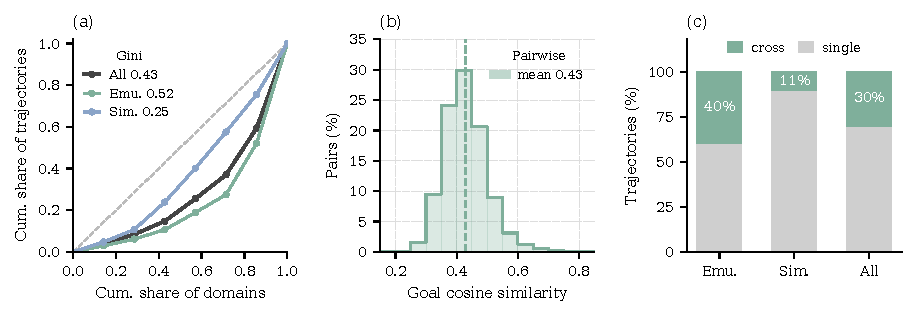
\includegraphics[
        width=\linewidth
    ]{figures/data-quality-3panel.pdf}
\caption{Diversity and coverage of OpenMobile-Data-v2.
\textbf{(a)}~Domain distribution across seven categories for emulator and simulator data. Gini coefficients quantify domain balance.
\textbf{(b)}~Pairwise cosine similarity among task goals.
\textbf{(c)}~Single-app and cross-app workflow composition.}
\label{fig:data-quality}
\end{figure}

OpenMobile-Data-v2 is diverse along three dimensions: domain distribution,
task diversity, and workflow diversity (Figure~\ref{fig:data-quality}).
The data span seven domains with a relatively balanced distribution. We quantify domain balance using the Gini coefficient, where lower values indicate more uniform coverage. The full set achieves a Gini coefficient of 0.43, while the emulator subset is more concentrated (0.52) and simulated clients provide more balanced coverage (0.25).
Task goals also show diversity, with a mean pairwise cosine
similarity of 0.43, indicating varied requests without excessive repetition.
Finally, the data cover both single-app and cross-app workflows, with 30\%
of trajectories spanning multiple applications (40\% on the emulator and
11\% on simulated clients). Together, these statistics show that
OpenMobile-Data-v2 provides diverse domains, task goals, and interaction
workflows.
